\documentclass{article}
\usepackage{graphicx}
\usepackage{amsmath}
\input defs.tex

\title{Project Report}
\author{Jesse Lu}
\begin{document}
\maketitle
\tableofcontents

\section{Main result: Quasi pareto-optimal portfolios}

    The main result of this project is the production of 
        eight portfolio groups with reduced turnover.
    What makes each portfolio group unique is the number of signals
        used to generate the portfolios in each group;
        for this project this was varied from 1 to 128 signals.
    Furthermore, within a portfolio group, 
        each portfolio is distinguished by its emphasis on maximizing
        either the annualized return, or information ratio.
    These results are presented in figure~\ref{result},
        as well as tables~\ref{table:ret}-\ref{table:tvr}.

    Surprisingly, these 

    \begin{figure}[t]
        \centerline{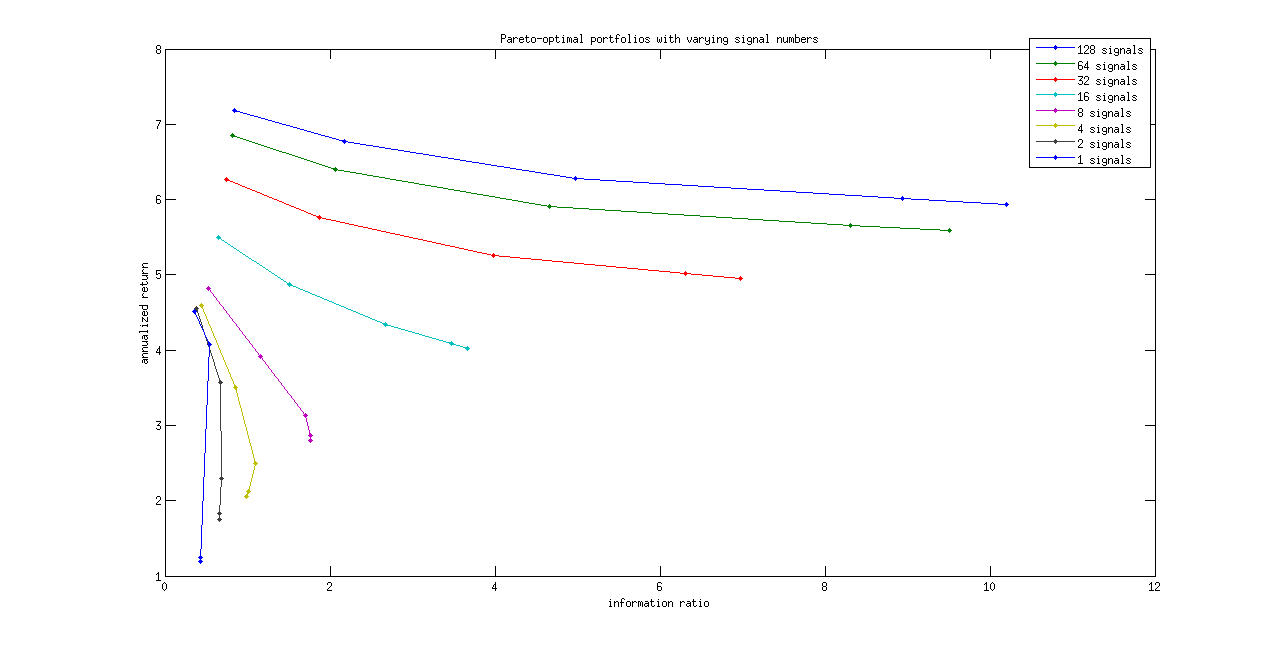
\includegraphics[width=1.8\textwidth]{result.png}}
        \caption{The main result of the project: 
                quasi pareto-optimal portfolios with varying numbers of signals,
                where even small signal numbers can produce large returns
                with large information ratios.
            Here, each point represents a portfolio, 
                while lines connect portfolios 
                generated by models of the same number of signals.
            The variety of portfolios for each signal number group
                is due to differentiated weighting between maximizing
                either the annualized return or the information ratio.
            }
        \label{result}
    \end{figure}
    \clearpage

    \begin{table}[t]\centering
        \begin{tabular}{l c c c c c c c c}
        $n_\text{signals}$ & 1 & 2 & 4 & 8 & 16 & 32 & 64 & 128  \\ \hline
        & 4.519 & 4.548 & 4.591 & 4.819 & 5.501 & 6.271 & 6.848 & 7.182  \\
        & 4.075 & 3.574 & 3.500 & 3.922 & 4.876 & 5.767 & 6.406 & 6.768  \\
        & 1.187 & 2.290 & 2.497 & 3.138 & 4.339 & 5.263 & 5.909 & 6.275  \\
        & 1.241 & 1.824 & 2.127 & 2.869 & 4.086 & 5.020 & 5.654 & 6.011  \\
        & 1.252 & 1.749 & 2.051 & 2.794 & 4.018 & 4.952 & 5.583 & 5.939 
        \end{tabular}
        \caption{Annualized returns of portfolios in figure~\ref{result}.}
        \label{table:ret}
    \end{table}

    \begin{table}[t]\centering
        \begin{tabular}{l c c c c c c c c}
        $n_\text{signals}$ & 1 & 2 & 4 & 8 & 16 & 32 & 64 & 128  \\ \hline
        & 0.348 & 0.375 & 0.425 & 0.513 & 0.641 & 0.739 & 0.801 & 0.837  \\
        & 0.533 & 0.661 & 0.848 & 1.149 & 1.500 & 1.864 & 2.054 & 2.161  \\
        & 0.421 & 0.679 & 1.083 & 1.691 & 2.664 & 3.968 & 4.650 & 4.965  \\
        & 0.416 & 0.655 & 0.999 & 1.759 & 3.466 & 6.304 & 8.300 & 8.933  \\
        & 0.413 & 0.654 & 0.980 & 1.756 & 3.656 & 6.972 & 9.504 & 10.200 
        \end{tabular}
        \caption{Information ratios of portfolios in figure~\ref{result}.}
        \label{table:ir}
    \end{table}


    \begin{table}[t]\centering
        \begin{tabular}{l c c c c c c c c}
        $n_\text{signals}$ & 1 & 2 & 4 & 8 & 16 & 32 & 64 & 128  \\ \hline
        & 0.163 & 0.159 & 0.151 & 0.142 & 0.148 & 0.163 & 0.175 & 0.183  \\
        & 0.131 & 0.123 & 0.116 & 0.114 & 0.130 & 0.153 & 0.170 & 0.179  \\
        & 0.061 & 0.084 & 0.082 & 0.095 & 0.122 & 0.149 & 0.168 & 0.178  \\
        & 0.058 & 0.073 & 0.071 & 0.090 & 0.120 & 0.148 & 0.168 & 0.177  \\
        & 0.058 & 0.071 & 0.069 & 0.089 & 0.119 & 0.148 & 0.167 & 0.177 
        \end{tabular}
        \caption{Turnover of portfolios in figure~\ref{result}.}
        \label{table:tvr}
    \end{table}

 \clearpage
\section{Finding the near-optimal forward-biased portfolio}

\subsection{Problem statement}
    The portfolio optimization problem can be simplified 
        by substituting expressions for the relevant terms in the following way
        (implemented in \verb+simulate_X.m+):
    \EE{}{
        f_{ir}(x) &= \frac{c^T x}{\std(Ax)} \\
        f_{ret}(x) &= a \frac{c^T x}{\norm{x}_1} \\
        f_{tvr}(x) &= \mean\frac{C|Bx|}{C|x|} \\
        f_{t}(x) &= \frac{\norm{Bx}_1}{\norm{x}_1}} 
    where for an $m$ stocks by $n$ days portfolio,
        \BI $x \in \reals^{mn}$ is a vector representing the portfolio,
        \I  $c$, $a$, $A$, $B$ and $C$ are appropriate vector, scalar, 
            or matrix quantities (see \verb+sim_matrices.m+), and
        \I  $f_{ir}, f_{ret}, f_{tvr}, f_{t} \in \reals^{mn} \to \reals$
            where $f_{t}$ is an approximation of the turnover function, 
            $f_{tvr}$. \EI

    The problem we want to solve is then
    \EE{original problem}{
        \minimize& - f_{ret}(x) - \hat{\mu}f_{ir}(x) \\
        \subto& f_{tvr}(x) \le 0.2
    }
    That is to say, maximize the return and information ratio
        (with relative proportion affected by coefficient $\hat{\mu}$)
        while keeping the turnover below $0.2$.


    Note that for brevity, I have not included the expressions for 
        $c$, $a$, $A$, $B$ and $C$; 
        however, one can deduce that such quantities must exist.
    For example, notice that $c^T x$ represents the total profit/loss;
        we know this expression must be valid for some $c$ 
        since the expression for the total profit/loss is linear.
    Lastly, notice that the portfolio is represented as a vector ($x$),
        rather than a matrix, in this section for notational convenience.

\subsection{Problem simplification}
    We now simplify \eq{original problem} in order 
        to make it computationally tractable.

    We first note that \eq{original problem} is homogenous,
        meaning that it's solution depends only on the relative values of $x$.
    Therefore we can split the terms of $f_{tvr}(x)$ in the following way
        without loss of generality.
    \EE{}{
        \minimize& - f_{ret}(x) - \hat{\mu}f_{ir}(x) \\
        \subto& \norm{Bx}_1 \le 0.2 \\
            & \norm{x}_1 = 1
    }

    Turning our attention to the objective function we note that
    \E{}{
        f_{ret}(x) + \hat{\mu}f_{ir}(x) = 
            \frac{c^T x}{\std(Ax)} + \hat{\mu} a c^T x}
        since $\norm{x}_1 = 1$.
    This objective can be thought of as 
        weighting two terms by $\hat{\mu}$;
        and we can alternatively weight the following two terms
    \E{}{
        \frac{c^T x}{\std(Ax)} + \hat{\mu} a c^T x \to 
            (1/\mu)c^T x - \std(Ax)}
        while still obtaining the full range of pareto-optimal points;
        although the connection between $\mu$ and $\hat{\mu}$
        is not immediately clear.

    This now gives us
    \EE{}{
        \minimize& (-1/\mu)c^T x + \std(Ax) \\
        \subto& \norm{Bx}_1 \le 0.2 \\
            & \norm{x}_1 = 1
    }
        which is still completely equivalent to \eq{original problem}.

    We now implement the following generalization
    \E{}{   \norm{x}_1 = 1 \quad\to\quad \norm{x}_1 \le 1}
        in order to make the problem 
        convex\footnote{see Boyd and Vandenberghe, ``Convex Optimization''}.
    Our reasoning behind this approximation
        is that although $\norm{x}_1$ is no longer 
        strictly confined to the value of 1,
        it most likely will end up with a quantity of 1 anyways
        because the $c^T x$ term in the objective function will always want
        to ``push'' $\norm{x}_1$ to as large a value as possible.

    While this approximation does inject error into our formulation,
        the benefits of convexity (i.e. the ability to efficiently compute
        the global minimum) far outweigh the costs.
    Actually, the cost of this approximation can be made negligible by
        twiddling the value of $0.2$ 
        in the $\norm{Bx}_1 \le 0.2$ constraint 
        (using a simple algorithm like bisection for instance)
        in order to force $f_{tvr}(x) \le 0.2$.
    
    We have now simplified \eq{original problem} into the following convex form
    \EE{convex problem}{
        \minimize& (-1/\mu)c^T x + \std(Ax) \\
        \subto& \norm{Bx}_1 \le 0.2 \\
            & \norm{x}_1 \le 1
    }
    
    

\end{document}
